\chapter{System Overview}
\label{cap3:system}
In this chapter we describe the main components of the proposed Question Answering system. 
First we briefly provide a general overview of the proposed system structure, and then explain 
in more detail each of the modules implemented for this work.

\section{Question Answering general overview}
\label{cap3:system/qaPipeline}
The Question Answering pipeline is divided into different stages, as seen in 
Figure~\ref{fig:questionAnsweringOverview}, which do not differ much from the standard 
Question Answering pipeline described by Lopez et al.~\cite{qa:core-techniques-DiefenbachLSM18}. 
We assume that the target Knowledge Graph is Wikidata for the purposes of the example, but 
the architecture can be applied more generally to any Knowledge Graph. For the question 
\dquotesit{Was Gabriela Mistral a poet?}, the expected answer can be retrieved from the 
Wikidata query service by executing an ASK-type \SPARQL{} query. In other cases a SELECT query may be 
required.

In order to build this \SPARQL{} query, the Question Answering system starts with an Entity 
Linking stage where relevant entities are identified (e.g., \dquotesit{Gabriel Mistral}, 
\dquotesit{poet}) and linked to the Knowledge Graph. Then, a Query Template Generation stage 
is performed to generate \SPARQL{} Query Template candidates with placeholders to be filled 
using the entities recognized in the previous stage. Next, a Slot Filling stage comes to 
identify which entities should be used to fill which placeholders of the query template 
candidates. This pipeline describing the Question Answering system is implemented by building 
three modules that perform each one of the described stages. 

\newpage

\begin{figure}[!h]
    \centering
    \includegraphics[scale=.5]{imagenes/3_system_overview/QuestionAnsweringPipeline.png}
    \caption{Question Answering system pipeline.}
    \label{fig:questionAnsweringOverview}
\end{figure}

\section{Query Generation Module}
\label{cap3:system/queryGenModule}
In this section we describe the Query Generation Module, which is used by the Baseline system 
and adapted for the system proposed in this work. Given a Natural Language (NL) question, the 
goal is to generate its logical form in terms of \SPARQL{} grammar, which can be either a 
complete \SPARQL{} query representation (baseline) or an intermediate Query Template 
representation (our system). 

We now explain the main components that encapsulate the Query Generation module. First, we 
describe the Query Generation pipeline, which does not differ much between the generation of 
an entire \SPARQL{} query or its Query Template. Then, we explain the Query Encoding used to 
deliver a normalized expression of the expected output for the model that performs the 
generation process. Finally, we describe in more detail how the model is trained and used to 
generate queries based on the FairSeq library for implementing Sequence to Sequence models in 
Python.

\subsection{Query Generation pipeline}
\label{cap3:system/queryGenModule/pipeline}
This module addresses two different tasks: translation from NL to \SPARQL{} queries, and 
generation of query templates from NL. 

On one hand, when we refer to \SPARQL{} queries, we refer to complete queries with all the 
entities, properties, \SPARQL{} keywords and operators necessary to be executable on any 
Wikidata endpoint. Previous works on this task are usually based on Sequence-to-Sequence 
models, where many have SQL as their target language~\cite{nmt:DongL16, nmt:CaiXZYLL18, 
nmt:ZhongCoRR17}. Most recent works apply similar models targeting \SPARQL{}~\cite{nmt:CoRRLuz18, 
nmt:nspm-SoruMMPVEN17, nmt:CoRRSoru18}.

On the other hand, Query Templates refer to intermediate representations of \SPARQL{} queries, 
which instead of containing the necessary entities included in a complete \SPARQL{} query, 
contain placeholders that will be later filled using the entities obtained in the Entity 
Linking stage. An example of both cases can be found in Figure~\ref{fig:queryGenerationOverview}, 
where the left side shows a \SPARQL{} query, and the right side its Query Template. 

\begin{figure}[!h]
    \centering
    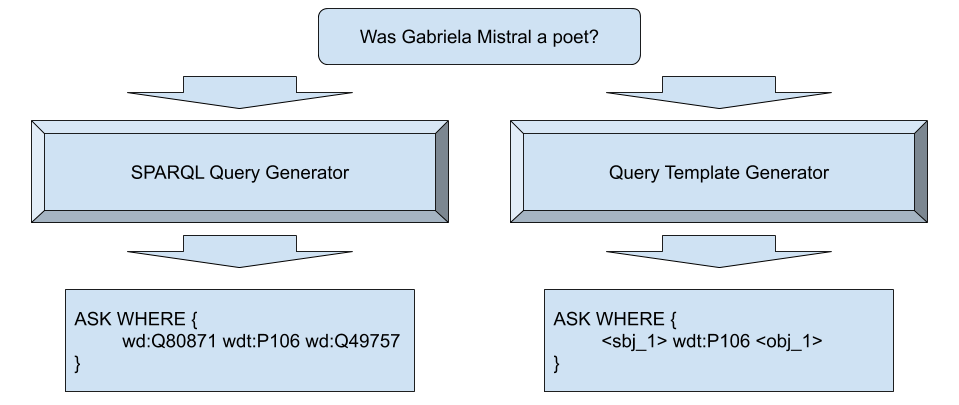
\includegraphics[scale=.5]{imagenes/3_system_overview/queryGenerationPipeline.png}
    \caption{Query Generation pipeline example.}
    \label{fig:queryGenerationOverview}
\end{figure}

In Figure~\ref{fig:queryGenerationOverview}, we can see the Query Generation pipeline and 
expected output for both tasks given the input NL question \dquotesit{Was Gabriela Mistral a 
poet?}. On the left, the \SPARQL{} query pipeline outputs an ASK-type \SPARQL{} question with two 
entities involved. On the other side, a Query Template is returned, which looks like an 
ASK-type \SPARQL{} query but it replaces the entities for two placeholders indicating that there 
is a subject entity and an object entity expected in the first triple of the Query Clause. 
The idea of the Query Template is that these placeholders will later be filled by the Slot 
Filling module.

As we mentioned before, the Query Generation pipeline does not change whether the model is 
generating an entire \SPARQL{} query or just an intermediate Query Template, and there are two 
reasons that explain this. First, both tasks can be seen as translating NL to a meaning 
representation, where such representations only vary on the information they are displaying. 
While generating a \SPARQL{} query includes the entities involved in the query, the generation 
of a Query Template replaces those entities for placeholders indicating that in those places 
an entity or a plain value will be needed, without specifying which ones. The second reason 
is that both models rely on the same data: a set of pairs of NL questions and \SPARQL{} queries. 
The only difference is that the output data used for the Query Template model is adapted to 
fit the Query Template generation task, where entities and plain values (e.g. numbers or 
strings values) are replaced by a placeholder that keeps a certain degree of information for 
the replaced value (e.g. placeholder type, query triple position, etc). This dataset 
adaptation process is explained in more detail in the \textit{Experimental Design} chapter~\ref{cap4:experimentalDesign}.

Aside from the input and output process, there are some intermediate steps performed over the 
input and output data. In the case of the input NL questions, a normalization process is 
conducted where the question string is lower-cased and non-relevant symbols are removed. On 
the output side, an encoding process is performed over the data used for training, and a 
decoding process is done for the query string output by the Query Generator system. The Query 
Encoding is done by tokenizing the \SPARQL{} grammar, allowing to treat it as a target wordy 
language, following the idea of reducing this problem to a Machine Translation task used in 
previous works~\cite{semPar:ChoMGBBSB14, semPar:sempar-as-mt-AndreasVC13, nmt:nl-to-sparql-Yin19}. 
Then, each of the two Generator models shown in Figure~\ref{fig:queryGenerationOverview} 4 
corresponds to a previously trained Fairseq model, which receives a normalized NL question 
and returns an encoded meaning representation that has to be later decoded to obtain the 
final \SPARQL{} query or Query Template output.

\subsection{Query Encoding}
\label{cap3:system/queryGenModule/encoding}
Following the same encoding approach used by Soru et al.~\cite{nmt:nspm-SoruMMPVEN17}, we 
encode the \SPARQL{} queries into tokens that describe entities, keywords, symbols, and 
operations. One difference is that we are using a dataset that includes new query components 
such as numbers or string values; thus we proposed novel tokens to encode those values. An 
example of this encoding can be seen in Listing~\ref{lst:encodingSPARQLSoru}. The main advantage of 
this encoding is that it allows the system to express chunks of commonly used patterns (e.g. 
order by asc/desc, or filter patterns) in a simpler way, thus reducing the complexity of the 
translation task.

\begin{sparqlcode}[%
    caption={\SPARQL{} query example with its encoded form.}, 
    label={lst:encodingSPARQLSoru}]
ASK WHERE { wd:Q658 wdt:P1108 ?obj FILTER(?obj < 1.2) }

ask where brack_open wd_q658 wdt_p1108 var_obj filter attr_open var_obj math_lt 1_dot_2 attr_close brack_close
\end{sparqlcode}

Query Templates are encoded in a similar way, but instead of encoding entities, numbers or 
string values, placeholders are used to replace those values. Besides those components, there 
is no other difference in the encoding process. Listing~\ref{lst:encodingTemplateSoru} shows 
the Query Template of Listing~\ref{lst:encodingSPARQLSoru} and its encoded form.

\begin{sparqlcode}[%
    caption={\SPARQL{} query example with its encoded form.}, 
    label={lst:encodingTemplateSoru}]
ASK WHERE { <sbj_1> wdt:P1108 ?obj FILTER(?obj < <num>) }

ask where brack_open placeholder_sbj_1 wdt_p1108 var_obj filter attr_open var_obj math_lt placeholder_num attr_close brack_close
\end{sparqlcode}

Note that instead of using letters for naming each placeholder as done by Ying et al.~\cite{nmt:nl-to-sparql-Yin19} 
(e.g. \texttt{A}, \texttt{B} or \texttt{C}) we use labels that provide more information about 
placeholders. For example, we identify placeholder type (subject, object, string value or 
numeric value) and position for entities placeholder (e.g. \texttt{sbj\_1} corresponds to the 
subject of the first triple in the Query clause).

These placeholder labels are also used in the Slot Filling system mentioned later in order to 
identify which entities output by the Entity Linking system corresponds to each one of the 
Query Template placeholders. 

\subsection{Fairseq Model}
\label{cap3:system/queryGenModule/fairseqModel}
The Query Generation model is implemented using the \textit{Facebook AI Research Sequence-to-Sequence 
Toolkit} (Fairseq), which implements various Seq2seq models based on Pytorch. Fairseq 
provides various off-the-shelf implementations and other settings to configure user 
experiments. 

In particular, we use the Convolutional Sequence to Sequence model (ConvS2S)~\cite{nmt:convS2S-GehringAGYD17} 
implementation to build the Query Generator model. The decision to use the ConvS2S is based 
on the work done by Yin et al.~\cite{nmt:nl-to-sparql-Yin19}, where eight Sequence-to-Sequence 
models were implemented and compared regarding the NL-to-SQL task. From this comparison, 
the ConvS2S model ended up having the best performance in terms of perplexity, BLEU score, 
and string-match accuracy. This model has to be trained and can be used later to generate an 
output depending on the given data. If we need to build a \SPARQL{} Query generator, we have to 
feed the system with pairs of NL questions and \SPARQL{} queries. In the same way, for a Query 
Template generator we instead use query templates as our output examples for training.

We now explain the main components of the ConvS2S architecture, the hyperparameters used with 
their values, and other training settings relevant to comprehend the training process. Note 
that the architecture used and its configuration is done following the work from 
Yin et al.~\cite{nmt:nl-to-sparql-Yin19}.

The ConvS2S architecture components used are based on the best-performance settings for 
natural language NMT~\cite{nmt:nl-to-sparql-Yin19}. In particular, the most relevant 
hyperparameters are the followings:

\begin{itemize}
    \item The number of \textbf{layers} used for the convolutional encoder and decoder is 15. 
    From these layers, the first 9 layers use 3x3 kernels with 512 units, the next 4 layers 
    use 3x3 kernels with 1024 units, and the final 2 layers uses a 1x1 kernel with 2028 units.
    \item The \textbf{optimizer}, i.e. the learning algorithm used, is Stochastic Gradient 
    Descent with minibatches. The default minibatch size is 64.
    \item The \textbf{learning rate} is set to fixed value of 0.5, which is maintained during 
    the entire training session.
    \item As a regularizer, \textbf{dropout} is applied with a fixed value of 0.2.
\end{itemize}

Besides those parameters, the Multi-step Attention mechanism is applied to some layers. The 
loss function used is the cross-entropy function mentioned in the \textit{Theoretical 
Framework} chapter~\ref{cap2:theoFrame/semPar/seq2seq}.

The training process is performed using Google Colaboratory, an online research tool that 
allows for writing and executing Python code and provides free computational resources, such 
as GPUs, to boost the training process. It is mainly focused on developing machine learning 
tasks. We also follow the same dataset split used by Yin et al.~\cite{nmt:nl-to-sparql-Yin19}: 
80\% for training and 20\% for dev/test. One difference is we only use train and dev sets, 
since other datasets are proposed as test sets. We chose this strategy as some of the 
existing datasets we use contain related or paraphrased questions, where creating an 
independent test set ensures that test questions are not derived from, or variants of, 
training questions. Each model is trained for a maximum amount of 40 epochs, where after 
every epoch a checkpoint is saved. Then, the checkpoint that achieves the lowest loss value 
for the validation set is kept.

The best values obtained from the training process can be imported later to the same Fairseq 
model implementation to perform new evaluations. When decoding on the evaluation stage, beam 
search is applied with a beam width of 5. As a last note, the same normalization process done 
for the training data has to be done with every new NL question. On the other hand, to obtain 
the \SPARQL{} query or the Query template it is always necessary to perform the decoded process 
over the Query Generator output.

\section{Entity Linking Module}
\label{cap3:system/entLinModule}
Two types of Entity Linking systems are considered for this work: Individual Entity Linking 
systems and Ensemble Entity Linking systems. First we discuss the pipeline that these systems 
follow.

\subsection{Entity Linking pipeline}
\label{cap3:system/entLinModule/pipeline}
An example for the Entity Linking pipeline is shown in Figure 2, for the question \dquotesit{Was 
Gabriela Mistral a poet?}. We assume that the Entity Linking module is available through an 
API; the Entity Linking system first retrieves the annotations by querying the API service, 
which returns annotations along with extra information (e.g. scores, second ranking entities, 
etc). In the case that the Entity Linking system targets a different Knowledge Graph to the one 
over which questions are answered, in a second (optional) phase the entities are mapped from 
the former to the latter (we do not compute the mapping in this work but rather assume that a 
mapping is made available).

\begin{figure}[!h]
    \centering
    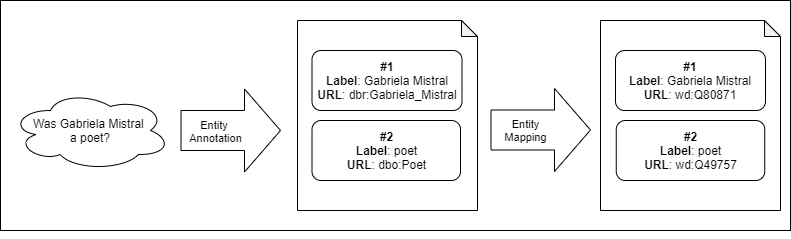
\includegraphics[scale=.5]{imagenes/3_system_overview/individualEntityLinkingPipeline.png}
    \caption{Entity Linking pipeline example.}
    \label{fig:entityLinkingPipeline}
\end{figure}

In this example, we show for each spotted mention: the start and end position, the annotation 
label and its associated resource. Then, an entity mapping process is performed to convert 
the DBpedia resources (\texttt{dbr:Gabriela\_Mistral} and \texttt{dbo:Poet}) into Wikidata 
resources (\texttt{wd:Q80871} and \texttt{wd:Q49757} respectively). As we mentioned, this 
mapping is optional and it depends on the target Knowledge Graph we are interested in, which 
in this case is Wikidata, and whether the system returns entities on that target Knowledge 
Graph.

The API service input parameters and output format is different for each web service, though 
the final output annotations from the Entity Linking module is always the same. An additional 
piece of information that is also returned are the scores each system gives to each annotation. 
Though these scores cannot be compared across systems, such scores are used to establish 
which entities are more relevant for each system. 

The Entity Mapping process assumes an existing mapping between the entities of both Knowledge 
Graphs. In this particular case, we can take advantage of the fact that many DBpedia resources 
and Wikidata resources are both bound to Wikipedia articles via the \texttt{schema:about} property. 
This information can be found on Wikidata, thereby, given a set of DBpedia entities, a \SPARQL{} 
query can be performed to retrieve their corresponding Wikipedia article and their related 
Wikidata entities, if any. An example of a \SPARQL{} query to map DBpedia entities to Wikidata 
ones can be seen in Listing~\ref{lst:entityMappingExample}.

\begin{sparqlcode}[%
    caption={\SPARQL{} query example to map DBpedia resources to Wikidata ones.}, 
    label={lst:entityMappingExample}]
SELECT ?article ?wikidata ?dbpedia WHERE {
    ?article schema:about ?wikidata .
    BIND(IRI(CONCAT("https://en.wikipedia.org/wiki/", SUBSTR(STR(?dbpedia),29))) AS ?article)
    VALUES ?dbpedia { <http://dbpedia.org/resource/Gabriela_Mistral> <http://dbpedia.org/ontology/Poet> }
}
\end{sparqlcode}

Following the same logic, Wikipedia articles can be mapped to its associated Wikidata resource. 
The opposite mapping from Wikidata resources to DBpedia ones can be easily performed as well. 
If any entity cannot be mapped from the results of the Entity Linking system to the target 
Knowledge Graph, it is discarded.

A final note about the entity mapping process is that it is performed over batches of entities, 
which means that a set of entities are mapped at the same time. This batch entity mapping is 
used to minimize the amount of queries done to the Wikidata query service. The final output 
values are returned in a JSON format.

\subsection{Individual Entity Linking systems}
\label{cap3:system/entLinModule/individualSystems}
We consider an Individual Entity Linking system as one of the Entity Linking systems mentioned 
in the Information Extraction chapter~\ref{cap2:theoFrame/infExtr/entityLinking}: 
DBpedia Spotlight~\cite{EL:dbpedia-spotlight-MendesJGB11}, 
AIDA~\cite{EL:aida-tool-YosefHBSW11, EL:aida-HoffartYBFPSTTW11}, TAGME~\cite{EL:tagme-FerraginaS10}, 
and OpenTapioca~\cite{EL:opentapioca-Delpeuch19}. These systems were selected because they 
provide public APIs that can be invoked over the Web. The annotation process is reduced to 
making a request on the corresponding API’s web service. We will briefly describe some details 
on the implementation and mention some aspects to take into consideration for each one of the 
aforementioned systems.

The \textbf{DBpedia Spotlight} system~\cite{EL:dbpedia-spotlight-MendesJGB11} aims to 
annotate DBpedia entities, so it requires a mapping process to convert the output annotations 
into Wikidata entities. The input parameters for the API request are the query text, a 
confidence value, and a support value. The confidence parameter is a threshold for disambiguation, 
and the support parameter is used to filter resources with a small number of Wikipedia 
inlinks. On the output side, DBpedia Spotlight assigns two scores to each entity: a 
similarity score, which represents how similar are the mention and the entity, and a 
percentage of second rank, which is the ratio of similarity scores between the second and the 
first candidates of the corresponding mention (used to measure the level of ambiguity for the 
mention).

The \textbf{AIDA} system~\cite{EL:aida-tool-YosefHBSW11, EL:aida-HoffartYBFPSTTW11} works over 
YAGO entities, though all YAGO entities map to a Wikipedia article. The annotations of this 
system can thereby be expressed as Wikipedia resources without the need for an extra query to 
the Wikidata query service. Nevertheless, the mapping process is done to map Wikipedia resources 
to Wikidata ones. Besides the text input parameter, the AIDA system does not require any other 
parameter. Each output annotation includes a disambiguation score which is the score assigned 
in the candidate ranking stage.

The \textbf{TAGME} system~\cite{EL:tagme-FerraginaS10} makes annotations over Wikipedia. As 
per AIDA, it requires a mapping stage to convert Wikipedia resources into Wikidata ones. 
Aside from the query text input parameter, TAGME requires a token parameter for authentication 
which can be retrieved from its API website. Each entity annotation has a \dquotesit{rho} score 
assigned, which is derived from the candidate ranking stage.

The \textbf{OpenTapioca} system~\cite{EL:opentapioca-Delpeuch19} is the only one that works 
directly over Wikidata. It does not require any extra parameter besides the query text. In 
the output annotation, a logarithmic likelihood score is assigned to each annotation, which 
points out how prominent the entity is in the Wikidata Knowledge Graph.

As a general aspect, the GET requests of most of the systems’ web services are done using the 
\texttt{request}\footnote{\url{https://pypi.org/project/requests/}} Python library, except for AIDA 
where \texttt{curl}\footnote{\url{https://curl.haxx.se/}} requests are done using the subprocess 
Python library. Then, the mapping queries performed on the Wikidata query service are done 
using the \texttt{SPARQLWrapper}\footnote{\url{https://pypi.org/project/SPARQLWrapper/}} Python 
library.

\subsection{Ensemble Entity Linking system}
\label{cap3:system/entLinModule/ensembleSystems}
Besides each individual Entity Linking system, we propose an ensemble of Entity Linking systems 
in order to improve the performance in terms of recognizing all the entities in a given 
question. Since each individual system relies on different techniques or prioritizes different 
features, they can identify entities that are either very prominent or quite rare. In the 
context of Question Answering, if an Entity Linking system cannot identify all of the entities 
needed to build the required \SPARQL{} query, the Question Answering system will fail to provide 
the right answer. The inability to identify all entities is more prone to happen when little 
context is provided in the given text, which is a common situation in Question Answering 
settings.

An ensemble Entity Linking system aims to get the most of all individual Entity Linking 
systems by combining their results together to achieve better Recall and Precision. Then, an 
ensemble system is given the annotations of each individual system as the system input and 
returns a final output annotation set. We present two variants to combine the individual 
annotations: Precision Priority system and Voting system. To illustrate better the variants 
proposed in this work, let us assume that each individual 
Entity Linking system returns the following annotations, for the question \dquotesit{Does FC 
Barcelona have Juan Jose Ibarretxe as a chairperson?}:

\newpage

\noindent \textbf{AIDA}\\
\mbox{}\\
\begin{sparqlcode}[]
FC Barcelona - wd:Q7156
\end{sparqlcode}

\noindent \textbf{OpenTapioca}\\
\mbox{}\\
\begin{sparqlcode}[]
Juan Jose Ibarretxe - wd:Q351738  
\end{sparqlcode}

\noindent \textbf{TAGME}\\
\mbox{}\\
\begin{sparqlcode}[]
Juan Jose Ibarretxe - wd:Q351738    
chairperson - wd:Q140686  
\end{sparqlcode}

\noindent \textbf{DBpedia Spotlight}\\
\mbox{}\\
\begin{sparqlcode}[]
Does - wd:Q302057
FC Barcelona - wd:Q7156
Juan Jose Ibarretxe - wd:Q351738
chairperson - wd:Q140686    
\end{sparqlcode}

After the description of each variant, an example of the expected output annotations is given 
based on the results shown above.

In this example, the annotations expected to be recognized are the entities from \dquotesit{FC 
Barcelona} and \dquotesit{Juan Jose Ibarretxe}. Even though some systems recognized 
\dquotesit{chairperson} as an entity, the property \dquotesit{chairperson} (\texttt{wdt:P488}) 
is more likely to be used when building the \SPARQL{} query for this question, so its entity is 
not expected to be identified. Though this ambiguity issue (whether something is a property or 
an entity) can complicate building the \SPARQL{} query, it is not something that we address in 
the Entity Linking stage. Returning more entities than the number expected is still acceptable 
as long as the correct entities are included among the output annotations. However, we will 
see in the \textit{Slot Filling module} section~\ref{cap3:system/slotFillModule} that the more 
entities are passed from the Entity Linking stage, the more difficult it can be to find the 
correct entity-placeholder mapping. Thus, a threshold can be set to define the number of 
expected entities, which is commonly the number of slots contained in the predicted Query 
Template.

\subsubsection{Precision Priority system}
\label{cap3:system/entLinModule/ensembleSystems/pprior}
The Precision Priority (PPrior) ensemble system establishes that some individual Entity 
Linking systems are more likely to return the expected answers, which in this case are the 
individual systems that tend to return fewer entities but with a high level of confidence, 
i.e. systems that prioritize Precision over Recall.

Then, the PPrior system assigns a priority to each individual system according to their 
performance on the datasets we are interested in (\LCQuADtwo, \DBNQA, and \QALDseven). In 
particular, systems with better precision have higher priority. These results can be found in 
the \textit{Results} chapter~\ref{cap5:results/entityLinking}, 
which establishes the following priority: AIDA, OpenTapioca, TAGME, and DBpedia Spotlight. Next, 
the PPrior system retrieves the annotations of each individual system following the established 
priorities until the number of unique expected entities is reached. 
For example shown above, the PPrior system would rank each entity in the following way:

\begin{sparqlcode}[]
1. FC Barcelona - Q7156
2. Juan Jose Ibarretxe - Q351738
3. chairperson - Q140686
4. Does - Q302057     
\end{sparqlcode}

The first entity (\texttt{Q7156}) comes from the AIDA system, the second one (\texttt{Q351738}) 
from OpenTapioca, the third one (\texttt{Q140686}) from one of the annotations output by 
TAGME (since the other entity has already been considered), and the remaining one (\texttt{Q302057}) 
comes from DBpedia Spotlight. Therefore, if the number of expected entities is two, the 
entities of the mentions \dquotesit{FC Barcelona} and \dquotesit{Juan Jose Ibarretxe} would be 
output as final annotations.

One advantage of this variant is that it would perform more efficiently in an online setting 
since it only requires to request annotations from the individual systems until it fulfills 
its expected number of entities. A disadvantage to take into consideration is that the PPrior 
system relies on the idea that systems with higher priority make fewer mistakes (e.g. 
recognize fewer false positives); thus incorrect entities from higher priority systems would 
have more value than correct entities from smaller priority systems.

\subsubsection{Voting system}
\label{cap3:system/entLinModule/ensembleSystems/voting}
The Voting ensemble system establishes a voting scheme where annotations from each individual 
system are considered to be a vote that is used to rank entities. This is based on the idea 
that if an entity is widely recognized across Entity Linking systems, that entity is more 
likely to be a correct annotation. Note that votes go for the entity identifier and not for 
the mention. Therefore, if two individual systems recognize the same entity but differ on the 
mentions linked, both systems are voting for the recognized entity (e.g. the \texttt{Q351738} 
entity could have been assigned to \dquotesit{FC Barcelona} or only to \dquotesit{Barcelona}, 
but votes go to the \texttt{Q351738} entity).

Given that ties are possible, the entities that come from more precise systems would have priority 
(following the same reasoning as with the PPrior system). For example, the Voting system 
would rank each entity in the following way:

\begin{sparqlcode}[]
1. (3) Juan Jose Ibarretxe - Q351738
2. (2) FC Barcelona - Q7156
3. (2) chairperson - Q140686
4. (1) Does - Q302057
\end{sparqlcode}

The most voted entity is \texttt{Q351738} with three votes, which comes from Open Tapioca, TAGME, 
and DBpedia Spotlight. Next, the entities \texttt{Q7156} and \texttt{Q140686} get the same 
amount of two votes. Since \texttt{Q7156} comes from a system with higher priority (AIDA), that 
entity ranks higher. The last entity \texttt{Q302057} only has one vote from the system with 
least priority (DBpedia Spotlight). Thereafter, if the number of expected entities is two, the 
entities of the mentions \dquotesit{Juan Jose Ibarretxe} and \dquotesit{FC Barcelona} would be 
output as final annotations.

The main advantage of the Voting system is that it can benefit from every system equally (all 
votes weigh the same regardless of their system’s precision). Thus, it seems reasonable to 
assume that the more systems are included in the voting process, the greater the chances are 
that the correct entities will be among the top voted ones. Some disadvantages are that with 
few systems the voting system does not differ much from the PPrior system, and its process is 
more expensive to execute since it always requires retrieving the annotations from all 
individual systems included.

\subsubsection{Other optimizations}
\label{cap3:system/entLinModule/ensembleSystems/optimizations}
In order to improve the performance of Ensemble Entity Linking systems, a couple of heuristic 
optimizations are proposed to achieve better performance. These improvements are included in 
the two variants mentioned before, and are optional features that can be skipped if no 
significant improvement is perceived. 

First, some entities linked to stopwords (e.g. \dquotesit{Does} linked to \texttt{Q302057}) are 
filtered using an English stopwords list provided by the Natural Language Toolkit\footnote{\url{https://www.nltk.org/}}. 
Before performing any join annotation process, the annotations that contain stop words are 
discarded. The idea behind this filter is to avoid entities from systems with low precision 
negatively affecting the identification of correct entities. However, some entities may 
include stopwords in their names (e.g. the rock band \dquotesit{The Who}), where this approach 
may negatively affect the results for such entities.

Lastly, a tiebreak system is implemented for entities that are ranked in the same position 
and come from the same system. Since each individual system assigns a score to each annotation, 
such scores can be used to break the tie and decide which entities will be considered in the 
final output. For example, if only two entities are expected but the second and third are 
tied (e.g. in the Voting system let us assume the entities from \dquotesit{Juan Jose Ibarretxe} 
and \dquotesit{chairperson} comes from OpenTapioca and have two votes each), we look at which 
has a higher score according to the individual Entity Linking system these annotations come from 
(i.e. which one has a higher \texttt{log\_likelihood} score according to OpenTapioca). 

\section{Slot Filling Module}
\label{cap3:system/slotFillModule}
In this section we describe the main components of the Slot Filling module, which is divided 
into two stages: the sequence labelling stage done by a Sequence Tagger, and the Query 
Filling stage where the spotted entities are filled into the given query template. We explain 
with details how the Slot Filling pipeline is structured, and then describe how the Sequence 
Tagger and the Query Filling algorithm are implemented.

\subsection{Slot Filling pipeline}
\label{cap3:system/slotFillModule/pipeline}
In Figure~\ref{fig:slotFillingPipeline}, we can see an overview of the Slot Filling process. 
Differently from the other modules, the Slot Filling system not only receives the input NL 
question, but also the outputs from the Entity Linking system and the Query Template generator. 
The expected output is a \SPARQL{} query which is based on the query template output by the 
Query Template generator, containing entities from the annotations returned by the Entity 
Linking system.

\begin{figure}[!h]
    \centering
    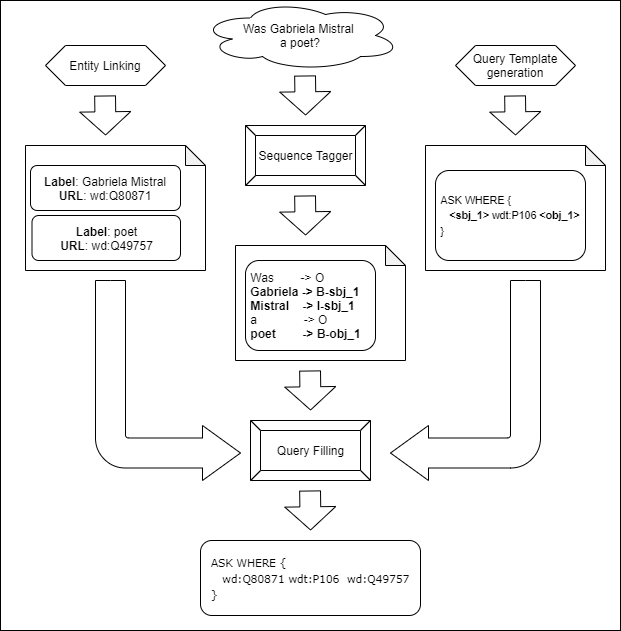
\includegraphics[scale=.5]{imagenes/3_system_overview/slotFillingPipeline.png}
    \caption{Slot Filling pipeline example.}
    \label{fig:slotFillingPipeline}
\end{figure}

Before the actual Slot Filling process, the input NL question is passed to a Sequence Tagger 
that performs Sequence Labelling in order to identify relevant named entities and their 
corresponding placeholder tag. We understand a placeholder tag as a placeholder name in a 
query template. As seen in Figure~\ref{fig:slotFillingPipeline}, given the question 
\dquotesit{Was Gabriela Mistral a poet?}, the expected output for the Sequence Tagger is to 
identify \dquotesit{Gabriela Mistral} and \dquotesit{poet} as two relevant entities. Besides, 
\dquotesit{Gabriela Mistral} is tagged as \dquotestt{sbj\_1}, meaning that the entity which 
corresponds to the label \dquotesit{Gabriela Mistral} should be assigned to the placeholder 
\texttt{<sbj\_1>} in the query template. The same happened with the label \dquotesit{poet}, 
which should be assigned to the placeholder \texttt{<obj\_1>}.

Then, the named entities tagged in the previous stage are passed to the Query Filling stage, 
along with the Entity Linking annotations and the generated Query Template. A filling 
algorithm is proposed to perform the Query Filling process. The algorithm will return a 
\SPARQL{} query only if the filling process is successful. As we will explain later, this filling 
process could fail due to the previous systems failing to recognize some entities, or due to 
a mismatch between the placeholders recognized in the tagging stage and the placeholder 
contained in the given query template.

\subsection{Sequence Tagger model}
\label{cap3:system/slotFillModule/seqTagger}
The Sequence Tagger identifies which named entities are more likely to have an entity 
assigned to a certain placeholder in the query template. To implement this model, we use the 
Flair\footnote{\url{https://github.com/flairNLP}} framework for Natural Language Processing. Flair 
contains many off-the-shelf Sequence Labelling and Name Entity Recognition models implemented 
using Pytorch. It also supports  training a custom Sequence Labelling model if training data 
is provided.

We then adapt the same dataset used for Query Generation to describe the expected output (more 
details in the \textit{Experimental design} chapter~\ref{cap4:experimentalDesign/datasets}). 
A Sequence Tagger model receives an NL 
question, and returns a sequence of tags where each tag is related to one word (or token) in 
the input question. These tags follow the BIO format, where each word is classified as the 
beginning of a tag, as the intermediate part of it, or as a non-tag token. For example, if 
given the question \dquotesit{Was Gabriela Mistral a poet?}, the expected output would be 
\texttt{(O, B-sbj\_1, I-sbj\_1, O, B-obj\_1)}. From this output we can infer that 
\dquotesit{Gabriela Mistral} is identified as one tag (\dquotesit{Gabriela} is the beginning of 
the tag and \dquotesit{Mistral} is an intermediate part of it), and \dquotesit{poet} is also 
identified as a tag. On the other hand, the words \dquotesit{Was} and \dquotesit{a} are identified 
as non-tag tokens. Note that the length of the tagger output and the number of tokens in the 
input question are always the same amount, so every token is assigned with a tag.

In this work three types of tag were chosen for three types of values: entities, numbers, and 
string values. The entity tag identifies entities from the Knowledge Graph resource (e.g. 
\texttt{wd:Q80871}). Each entity tag identifies two aspects of the entity: 1) its role in the 
query triple (subject or object), and its query triple position. For example, if an entity is 
tagged as \dquotestt{sbj\_1}, it means it is the subject of the first query triple. As their 
names may suggest, the number tag identifies numeric values, and the string value tag marks 
text relevant to the query (e.g. for filtering entities that contain a certain string label).

There are two main steps before training the Sequence Labelling Model: preprocessing the 
dataset, and configuring the model architecture. The Sequence Labelling dataset has to be 
converted to a tag dictionary that fits the Flair model input. Each output value has to be 
expressed as a sequence of BIO labels. Whatever BIO labels are chosen determines the labels 
the Sequence Tagger will use. Next, the configuration of the model architecture is divided 
into embeddings and model settings. First, the embedding layer is set, where one or more 
types of embeddings can be joined into a stacked embedding. In this case, we use the GloVe 
embeddings along with contextual embeddings known as Flair embeddings~\cite{seqlab:flair-AkbikBBRSV19}. 
Lastly, the model architecture used is the same standard architecture used by 
Akbik et al.~\cite{seqlab:contextual-emb-AkbikBV18}, which is a BiLSTM~\cite{seqlab:HuangXY15} 
with the number of hidden layers set to 256, along with a CRF layer put on top of the final 
layer. 

Finally, there are some training parameters or settings that are defined by default and 
others that can be tuned for a particular task. Some default aspects include the learning 
algorithm (mini-batch stochastic gradient descent) and the loss function (cross-entropy 
function). Some relevant training parameters that can be tuned are the learning rate, the 
minibatch size, and the number of epochs. The model is trained until it has a fixed number of 
epochs without an improvement in terms of loss value.

\subsection{Slot Filling method}
\label{cap3:system/slotFillModule/fillingMethod}
The placeholder tags for each named entity, along with the annotations from the Entity 
Linking system and the query template from the Query Template generator, need to be combined 
together to build the final \SPARQL{} query output. The Slot Filling method decides which 
placeholder to replace with which entity, and is based on a novel filling algorithm divided 
into two filling stages. The first stage is a \textbf{Standard Filling} process that may not 
fill all the placeholders in the query, and the second stage is a \textbf{Force Filling} 
process that tries to complete the spots that the previous stage was not able to fill.

The first stage, the Standard Filling process, follows a straightforward process of comparing 
labels from the outputs of the Entity Linking system and the Sequence Tagger to identify 
entity-slot matches which are then inserted into the query template to form the \SPARQL{} query. 
Then, the algorithm that describes the standard filling process is shown in 
Listing~\ref{lst:standardFillingAlgorithm}. As an example from the input shown in 
Figure~\ref{fig:slotFillingPipeline}, the algorithm would first compare the label 
\dquotesit{Gabriela Mistral} with all the labels from the entity annotations. Then, it would 
be found that the placeholder \texttt{sbj\_1} should correspond to the entity 
\texttt{wd:Q80871} given that both labels are equal. Based on this match, the entity 
\texttt{wd:Q80871} should replace all the appearances of the placeholder \texttt{sbj\_1} in 
the current \SPARQL{} query that is being constructed.

\begin{sparqlcode}[%
    caption={Standard Filling algorithm.}, 
    label={lst:standardFillingAlgorithm}]
standard_filling(annotations, slots, query_template)
    sparql_query = query_template
    for s_label, placeholder in slots
        if placeholder has been used or placeholder not in sparql_query
            skip
        if placeholder is a <num> or <str_value>
            replace placeholder in sparql_query for the s_label value
        if placeholder is an <entity_type> (e.g. <sbj_1>)
            for e_label, entity in annotations
                if s_label equal to e_label
                    replace placeholder in sparql_query for the entity value
                    break
        mark placeholder and/or entity as used, if applies
    return sparql_query
\end{sparqlcode}

Some problems can arise from this algorithm, which are mainly due to previous systems passing 
incorrect or incomplete information (e.g. not all the entity annotations are identified, or 
the Sequence Tagger tag some mentions incorrectly). Consequently, some placeholders may not 
be filled by the standard filling process. In such cases, a second filling process, called 
Force Filling, is performed to address these issues.

Force Filling aims to fill all slots in a best-effort manner, and is performed based on some 
assumptions and heuristics. The first assumption is that since we usually deal with short 
questions, the number of entities to be identified and placeholders to be filled tend to be 
low, not having more than three spots to fill in average. We also assume that most of the 
mistakes made by the Sequence Tagger are due to incorrect tagging. Also, multiple word labels 
from annotations and from the Sequence Tagger might differ but if they share one or more 
words, it is more likely that both labels refer to the same value. Lastly, we assume that if 
one spot is left to be filled, and one entity is left to be used, it is likely that that 
entity should be placed there even if the slot label and the entity label are not the same. 
Considering all that, the mistakes made by previous systems can be mitigated by using simple 
heuristic rules. 

To summarize, a similar filling process to the one shown in Listing~\ref{lst:standardFillingAlgorithm} 
is executed, but adding the following rules:
\begin{itemize}
    \item If any slot label is contained in an entity label (or vice versa), it counts as a 
    match.
    \item When comparing entity type placeholders, if the slot placeholder is the same entity 
    type (subject or object) or is assigned to the same query triple (e.g. the first query 
    triple pattern on the \SPARQL{} query) as some of the remaining query template placeholders, 
    it counts as a match.
    \item Finally, if there is any remaining entity that was not identified by the Sequence 
    Tagger, and there are still placeholders to fill in the query template, the entities will 
    be inserted in order until all spots have been filled (where the order is defined by the 
    entity identifier number).
\end{itemize}

As an example, let us assume we have the outputs illustrated in Figure~\ref{fig:forceFillingExample} 
for the question \dquotesit{How many Nobel Prizes has Gabriela Mistral won?}, which requires a 
count operation. The expected slots state that the subject of the first query triple should 
be filled with the entity of the label \dquotesit{Gabriela Mistral}, while the object of the 
second query triple should be filled with the entity of the label \dquotesit{Nobel Prizes}. 
However, it may happen that a label is incorrectly associated with the wrong query triple 
(case 1), or the wrong entity type (case 2). In the first case, the \dquotesit{Nobel Prizes} 
entity would not be filled in the Standard Slot Filling stage due to the \texttt{<obj\_2>} 
not existing in the query template, but it would be recognized in the Force Slot Filling 
stage because it will identify that the remaining slot in the query template (\texttt{<obj\_1>}) 
is the same entity type as the slot incorrectly labeled (\texttt{<obj\_2>}). The same happens 
in the second case, where the incorrect label (\texttt{<obj\_1>}) is associated with the same 
query triple (the first triple) as the remaining slot in the query template (\texttt{<sbj\_1>}).

\begin{figure}[!h]
    \centering
    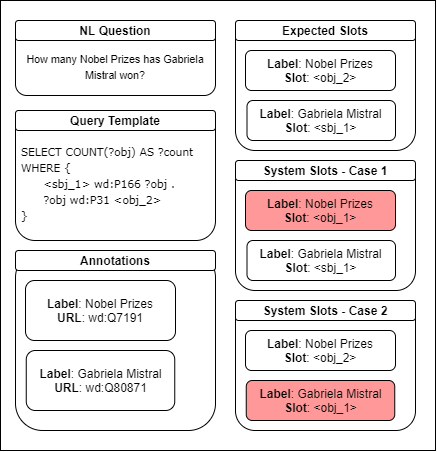
\includegraphics[scale=.5]{imagenes/3_system_overview/SlotFillingSpecialCases.png}
    \caption{Force Filling case examples.}
    \label{fig:forceFillingExample}
\end{figure}

Although more cases can be correctly filled by applying these rules, there are some other 
cases that are not possible to correctly fill. For example, the Sequence Tagger can identify 
the expected placeholder but it can wrongly associate each one to an incorrect mention (e.g. 
wrongly associate the subject entity and object entity of one query triple). A more serious 
case is when the Sequence tagger provides placeholders that have nothing to do with the ones 
found in the query template, usually because both systems identified a different intention in 
the given answer. In summary, the success rate of the filling process is strongly affected by 
the performance of the previous systems that deliver the input for this Slot Filling system.
